\documentclass[a4paper,12pt]{book}
\usepackage{ctexcap} % 是过时宏包。
\usepackage{amsmath} % AMS 数学公式扩展
\usepackage{graphicx} % 插入图片宏包
\usepackage{fancyhdr} % 设置latex页眉页角
\usepackage[super,square,comma,sort&compress]{natbib} % 设置參考文献的格式 角标直接在该文件中书写

\usepackage{geometry} % 设置页边距
\geometry{left=4cm,right=2cm,top=3cm,bottom=2cm} % 分别是左右上下

\newcommand{\tabincell}[2]{
    \begin{tabular}
        {@{}#1@{}}#2
    \end{tabular}}% 设置换行

\graphicspath{{pics/},{figs/}} % 图片在当前目录下的 pics和figs 目录

\usepackage{float} % 是图片悬浮
\usepackage{bm} % 字体加粗
\usepackage{times} 
\usepackage{mathptmx} % 设置为罗马体
\usepackage{caption} % 可以修改标题
\captionsetup{labelsep=space}
%\usepackage[colorlinks,dvipdfm,  %电子版时使用这个包
%            bookmarksopenlevel=2,
%            pdfpagemode=UseNone,
%            pdfstartview=FitB,
%            linkcolor=black,
%            citecolor=blue,
%            linkcolor=black,
%            hyperindex=true,
%            pagebackref=true,
%            CJKbookmarks=true,
%            colorlinks]{hyperref}

\renewcommand{\captionfont}{\zihao{5}\songti}
\renewcommand\theequation{\thechapter-\arabic{equation}} % 公式编号
\usepackage{setspace} % 使用间距宏包
\usepackage{comment}
\linespread{1.5} % 1到5章

\CTEXsetup[nameformat]{}
\CTEXsetup[beforeskip={0pt}]{chapter}
\CTEXsetup[nameformat={\heiti\zihao{3}\centering}]{chapter}%章标题格式
\CTEXsetup[titleformat={\heiti\zihao{3}\centering}]{chapter}%章标题格式
\CTEXsetup[format={\songti\zihao{4}\centering}]{section}% 节标题格式
\CTEXsetup[format={\songti\zihao{-4}}]{subsection}%小节标题格式
\CTEXsetup[format={\songti\zihao{-4}}]{subsubsection}%小节标题格式
\usepackage{titletoc} % 改变章节格式

\begin{document}\songti\zihao{-4}%设置正文字体格式


\pagenumbering{Roman} % 页面设置 罗马字体

\include{Abstract}
\songti\zihao{-4}
\setcounter{tocdepth}{2}%设置文件夹深度
\thispagestyle{plain}
\titlecontents{chapter}
              [0.0em]
              {\songti\zihao{-4}\bfseries\addvspace{10bp minus 0bp}}  %\song
              {\thecontentslabel\hspace{0.5em}}
              {}
              {\normalfont\dotfill\textrm{\contentspage[{\bfseries\thecontentspage}]}}
\newgeometry{bottom=3cm,top=3cm}
\tableofcontents % 生成一个目录
\restoregeometry



\chapter{绪论}
\section{研究背景及意义}
写下这句诗,我起身立于窗前。此刻,夜空如墨,夜空下的城市灯火阑珊,一幢幢居民楼灯火通明,闪闪烁烁如繁星沉醉,亦如我此刻变幻的思绪。那陌生而熟悉的事,那模糊而清晰的人,那温暖的微笑,那亲切的问候,如光似电,快速地在我的心湖湖面上,泛滥成灾。我刻意地捕捉,如捕捉一只只恣肆的蜻蜓、放纵的蝴蝶,希望她们的容貌能清晰些,再清晰些。
\subsection{无线频谱的分配与利用}
是你吗,那公交车上让座的温情?是你吗,那电梯门口等候的耐心?是你吗,那来自远方的贴心鼓励?是你吗,那扎着红丝带的生日祝福?是的,都是的,那么微弱,却又那么滚烫;那么遥远,却又那么真切,好似枕边的清凉,触手可及。让我们即使在清冷的夜里也能感觉到,人间至味。
\begin{figure}
    \centering
    \caption{这是第一张图片}
    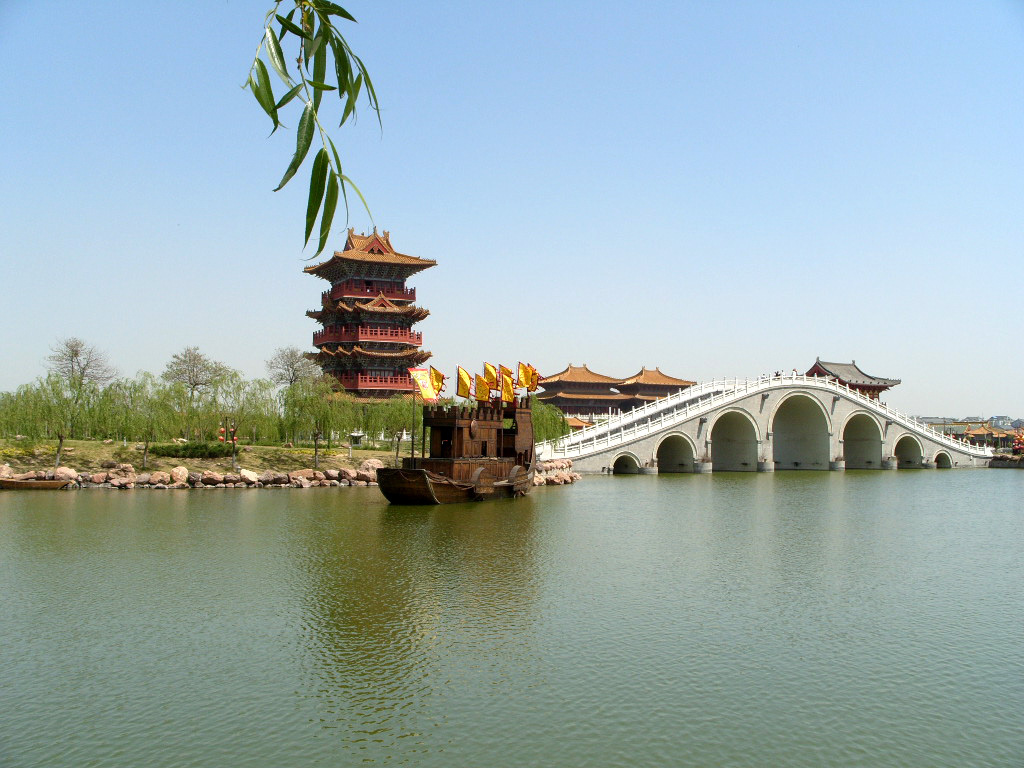
\includegraphics[scale=0.4]{figures/timg.jpg}
\end{figure}

\subsection{提高频谱利用效率的方法}
\begin{table}
    \centering
    \caption{这是第一个表格}
    \begin{tabular}{cccc}
        \toprule
        & \multicolumn{3}{c}{Numbers} \\
        \cmidrule{2-4}
        & 1 & 2 & 3 \\
        \midrule
        Alphabet & A & B & C \footnotemark \\
        Roman & I & II& III \\
    \bottomrule
    \end{tabular}
    
\end{table}
\footnotetext{表格里的字母是英文字母}
记忆伸向久远的过去,我再次触摸到你的呼吸。那是一个凄冷的早春,我身无分文,孑然立于城市街头。我在寒风中颤栗,也在寒风中绝望,我选择了一个失败者所能选择的结局:自杀 。当我横卧于铁轨上等待即将呼啸而至的列车时,你的强有力的大手一把把我拽离铁轨,并把我牵引入你的值班室。室内的炉火烘热了我的身体,你温润的话语烘热了我的心灵。我吃着你给我打来的饭菜,泪如雨下。你给了我五十块钱,劝我回家。最终你还是不放心,又一路陪同我到火车站,直到看着我进了站,你才放心离去
\section{认知无线电概述}
由于工作的关系,我和你被拉到同一个工作群里。我爱写作,每有新作出炉,总会发至群里供大家评点。你总是先给我回一串大大的赞,然后在软文后面写上你的阅读感受。一来二去,我们成了“朋友”。你说,你很敬佩我的高雅,想送给我一个礼物。我心生感动,但也只是当做逢场的恭维,不以为意。没想到,五天之后,我收到了来自你的快递。急急打开,原来是厚厚三大本书:日本儒学泰斗冈田武彦先生的心血力作《王阳明大传》全册。瞬间,我忍不住潸然泪下。不仅为你的倾心相赠,更为你的心细如发,我仅仅截图了我的电子书目发给你,里面有我喜欢的书《明朝一哥王阳明》,你竟然记住了。而今,我们依然是微信里的“朋友”,我只知道你是谁,你的名字叫赵冉,网名叫语冉心文。
\subsection{认知无线电的定义}
夜深沉,我却无心入睡。我于千里之外写下的关于你的文字,只为了让你知道,你如昙花一样惊艳的刹那芳华,已经深深绚烂了一颗孤独的心。你们不是这个社会的筋骨,但你们一定是这个社会的血肉
\subsection{认知无线电的关键技术}
风起叶落,年岁老去。这是在告诫人们,为什么不曾着此时拥有,好好把握属于自己的年华。秋风起时,不是单一用来相思和发愁的,而是用来思考和感悟的。



梧桐,银杏,合欢,秋天的风物在风中展示着自己的特性。城市与乡村,被任性的秋风抚摸。仿佛打翻了的调色盘,美丽的色彩把秋的意境拉长
\subsection{国内外认知无线电的研究现状}
乡间的落花生,砍高粱,掰玉米,割豆子,晒柿子。城市里,公园水边的芦苇在秋天诉说着,垂柳摆动着枝条,水草安静。出来散步的人群,吹着凉风,惬意而舒适,有人由衷说一句:“生活真的很美好!”



这么美好的生活,我们为什么要哀愁呢?应该尽情欢笑,尽管生活它有太多不如意,可是我们依旧满怀梦想。有梦就去追赶,趁着山高路长。尽管命运总是会捉弄人,可是我们依旧拥有爱与温暖。



路边的水吧,传来点唱机的音乐。秋风下,一点点灯火的昏黄,有着诗意的朦胧。此时此境,我路过它的美丽。不由得叹道:“人们总是渴望着诗和远方。却不能看见自己眼前的生活,就有着诗意的所在,和远方的期待。
\section{论文内容及结构}
\begin{figure}
    \centering
    \caption{这是第二张图片}
    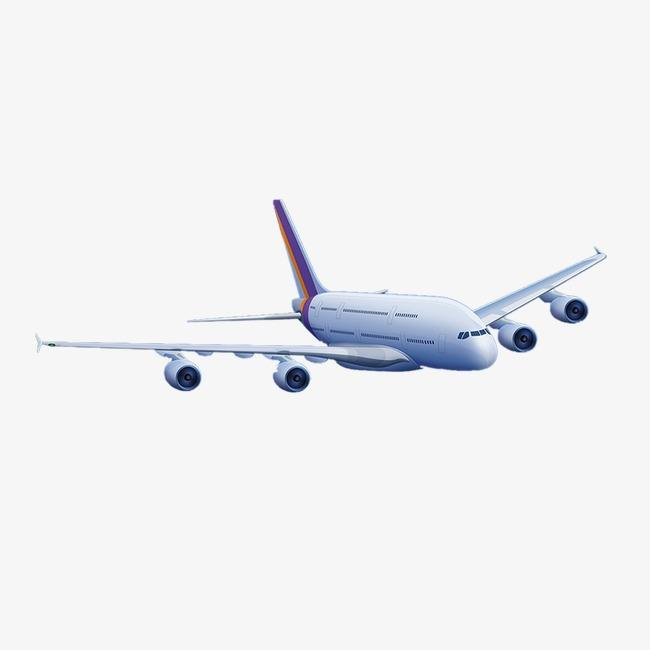
\includegraphics[scale=0.4]{figures/timg1.jpg}
\end{figure}
深有同感。多年前认识一个朋友,在外地工作。那时的联系方式主要是电话,原本节俭的他,却会在陌生的街头,日日给家中的妻儿挂一通电话。后来聚会时,他讲起自己的漂泊,说到此处,我们问为什么。



朋友很实在,他说:“这样我们一家人,会感觉每天生活在一起。”直至今天,我才读懂他对生活的理解。对生活深情的人,会在时间中种植深情。







秋风已起,思念与愁绪,深情与厚意,都在其中。我们都是风的孩子,乘着它的翅膀在人间飞翔。我时时告诫自己:“珍重待秋风!”
秋风已起,思念与愁绪,深情与厚意,都在其中。我们都是风的孩子,乘着它的翅膀在人间飞翔
秋风已起,思念与愁绪,深情与厚意,都在其中。我们都是风的孩子,乘着它的翅膀在人间飞翔秋风已起,思念与愁绪,深情与厚意,都在其中。我们都是风的孩子,乘着它的翅膀在人间飞翔
秋风已起,思念与愁绪,深情与厚意,都在其中。我们都是风的孩子,乘着它的翅膀在人间飞翔秋风已起,思念与愁绪,深情与厚意,都在其中。我们都是风的孩子,乘着它的翅膀在人间飞翔
秋风已起,思念与愁绪,深情与厚意,都在其中。我们都是风的孩子,乘着它的翅膀在人间飞翔秋风已起,思念与愁绪,深情与厚意,都在其中。我们都是风的孩子,乘着它的翅膀在人间飞翔
秋风已起,思念与愁绪,深情与厚意,都在其中。我们都是风的孩子,乘着它的翅膀在人间飞翔秋风已起,思念与愁绪,深情与厚意,都在其中。我们都是风的孩子,乘着它的翅膀在人间飞翔
秋风已起,思念与愁绪,深情与厚意,都在其中。我们都是风的孩子,乘着它的翅膀在人间飞翔
秋风已起,思念与愁绪,深情与厚意,都在其中。我们都是风的孩子,乘着它的翅膀在人间飞翔
秋风已起,思念与愁绪,深情与厚意,都在其中。我们都是风的孩子,乘着它的翅膀在人间飞翔
秋风已起,思念与愁绪,深情与厚意,都在其中。我们都是风的孩子,乘着它的翅膀在人间飞翔
秋风已起,思念与愁绪,深情与厚意,都在其中。我们都是风的孩子,乘着它的翅膀在人间飞翔
秋风已起,思念与愁绪,深情与厚意,都在其中。我们都是风的孩子,乘着它的翅膀在人间飞翔
秋风已起,思念与愁绪,深情与厚意,都在其中。我们都是风的孩子,乘着它的翅膀在人间飞翔秋风已起,思念与愁绪,深情与厚意,都在其中。我们都是风的孩子,乘着它的翅膀在人间飞翔
秋风已起,思念与愁绪,深情与厚意,都在其中。我们都是风的孩子,乘着它的翅膀在人间飞翔
秋风已起,思念与愁绪,深情与厚意,都在其中。我们都是风的孩子,乘着它的翅膀在人间飞翔
秋风已起,思念与愁绪,深情与厚意,都在其中。我们都是风的孩子,乘着它的翅膀在人间飞翔
秋风已起,思念与愁绪,深情与厚意,都在其中。我们都是风的孩子,乘着它的翅膀在人间飞翔
秋风已起,思念与愁绪,深情与厚意,都在其中。我们都是风的孩子,乘着它的翅膀在人间飞翔

秋风已起,思念与愁绪,深情与厚意,都在其中。我们都是风的孩子,乘着它的翅膀在人间飞翔
秋风已起,思念与愁绪,深情与厚意,都在其中。我们都是风的孩子,乘着它的翅膀在人间飞翔
秋风已起,思念与愁绪,深情与厚意,都在其中。我们都是风的孩子,乘着它的翅膀在人间飞翔
秋风已起,思念与愁绪,深情与厚意,都在其中。我们都是风的孩子,乘着它的翅膀在人间飞翔
秋风已起,思念与愁绪,深情与厚意,都在其中。我们都是风的孩子,乘着它的翅膀在人间飞翔
秋风已起,思念与愁绪,深情与厚意,都在其中。我们都是风的孩子,乘着它的翅膀在人间飞翔

秋风已起,思念与愁绪,深情与厚意,都在其中。我们都是风的孩子,乘着它的翅膀在人间飞翔
秋风已起,思念与愁绪,深情与厚意,都在其中。我们都是风的孩子,乘着它的翅膀在人间飞翔
秋风已起,思念与愁绪,深情与厚意,都在其中。我们都是风的孩子,乘着它的翅膀在人间飞翔
秋风已起,思念与愁绪,深情与厚意,都在其中。我们都是风的孩子,乘着它的翅膀在人间飞翔
秋风已起,思念与愁绪,深情与厚意,都在其中。我们都是风的孩子,乘着它的翅膀在人间飞翔
秋风已起,思念与愁绪,深情与厚意,都在其中。我们都是风的孩子,乘着它的翅膀在人间飞翔

秋风已起,思念与愁绪,深情与厚意,都在其中。我们都是风的孩子,乘着它的翅膀在人间飞翔
秋风已起,思念与愁绪,深情与厚意,都在其中。我们都是风的孩子,乘着它的翅膀在人间飞翔
  % 第一章
\chapter{绪论}
\section{研究背景及意义}
黑胡椒苦咖啡和哈弗卡积分换看哈复活卡就划分框架啊饿会儿话费发挥咖啡壶碍口发哈扣积分换
黑胡椒苦咖啡和哈弗卡积分换看哈复活卡就划分框架啊饿会儿话费发挥咖啡壶碍口发哈扣积分换
黑胡椒苦咖啡和哈弗卡积分换看哈复活卡就划分框架啊饿会儿话费发挥咖啡壶碍口发哈扣积分换
黑胡椒苦咖啡和哈弗卡积分换看哈复活卡就划分框架啊饿会儿话费发挥咖啡壶碍口发哈扣积分换
\subsection{无线频谱的分配与利用}
\subsection{提高频谱利用效率的方法}
\section{认知无线电概述}
\subsection{认知无线电的定义}
\subsection{认知无线电的关键技术}
\subsection{国内外认知无线电的研究现状}
\section{论文内容及结构}

%\chapter{议论过程}

那天读到一段话:“如果你爱的人就在身边,请一定好好抱紧她;
\section{研究背景及意义2}
写下这句诗,我起身立于窗前。此刻,夜空如墨,夜空下的城市灯火阑珊,一幢幢居民楼灯火通明,闪闪烁烁如繁星沉醉,亦如我此刻变幻的思绪。那陌生而熟悉的事,那模糊而清晰的人,那温暖的微笑,那亲切的问候,如光似电,快速地在我的心湖湖面上,泛滥成灾。我刻意地捕捉,如捕捉一只只恣肆的蜻蜓、放纵的蝴蝶,希望她们的容貌能清晰些,再清晰些。
\subsection{无线频谱的分配与利用2}
是你吗,那公交车上让座的温情?是你吗,那电梯门口等候的耐心?是你吗,那来自远方的贴心鼓励?是你吗,那扎着红丝带的生日祝福?是的,都是的,那么微弱,却又那么滚烫;那么遥远,却又那么真切,好似枕边的清凉,触手可及。让我们即使在清冷的夜里也能感觉到,人间至味。
\subsection{提高频谱利用效率的方法2}
记忆伸向久远的过去,我再次触摸到你的呼吸。那是一个凄冷的早春,我身无分文,孑然立于城市街头。我在寒风中颤栗,也在寒风中绝望,我选择了一个失败者所能选择的结局:自杀 。当我横卧于铁轨上等待即将呼啸而至的列车时,你的强有力的大手一把把我拽离铁轨,并把我牵引入你的值班室。室内的炉火烘热了我的身体,你温润的话语烘热了我的心灵。我吃着你给我打来的饭菜,泪如雨下。你给了我五十块钱,劝我回家。最终你还是不放心,又一路陪同我到火车站,直到看着我进了站,你才放心离去
\section{认知无线电概述2}
由于工作的关系,我和你被拉到同一个工作群里。我爱写作,每有新作出炉,总会发至群里供大家评点。你总是先给我回一串大大的赞,然后在软文后面写上你的阅读感受。一来二去,我们成了“朋友”。你说,你很敬佩我的高雅,想送给我一个礼物。我心生感动,但也只是当做逢场的恭维,不以为意。没想到,五天之后,我收到了来自你的快递。急急打开,原来是厚厚三大本书:日本儒学泰斗冈田武彦先生的心血力作《王阳明大传》全册。瞬间,我忍不住潸然泪下。不仅为你的倾心相赠,更为你的心细如发,我仅仅截图了我的电子书目发给你,里面有我喜欢的书《明朝一哥王阳明》,你竟然记住了。而今,我们依然是微信里的“朋友”,我只知道你是谁,你的名字叫赵冉,网名叫语冉心文。
\subsection{认知无线电的定义2}
夜深沉,我却无心入睡。我于千里之外写下的关于你的文字,只为了让你知道,你如昙花一样惊艳的刹那芳华,已经深深绚烂了一颗孤独的心。你们不是这个社会的筋骨,但你们一定是这个社会的血肉
\subsection{认知无线电的关键技术2}
风起叶落,年岁老去。这是在告诫人们,为什么不曾着此时拥有,好好把握属于自己的年华。秋风起时,不是单一用来相思和发愁的,而是用来思考和感悟的。



梧桐,银杏,合欢,秋天的风物在风中展示着自己的特性。城市与乡村,被任性的秋风抚摸。仿佛打翻了的调色盘,美丽的色彩把秋的意境拉长
\subsection{国内外认知无线电的研究现状2}
乡间的落花生,砍高粱,掰玉米,割豆子,晒柿子。城市里,公园水边的芦苇在秋天诉说着,垂柳摆动着枝条,水草安静。出来散步的人群,吹着凉风,惬意而舒适,有人由衷说一句:“生活真的很美好!”



这么美好的生活,我们为什么要哀愁呢?应该尽情欢笑,尽管生活它有太多不如意,可是我们依旧满怀梦想。有梦就去追赶,趁着山高路长。尽管命运总是会捉弄人,可是我们依旧拥有爱与温暖。



路边的水吧,传来点唱机的音乐。秋风下,一点点灯火的昏黄,有着诗意的朦胧。此时此境,我路过它的美丽。不由得叹道:“人们总是渴望着诗和远方。却不能看见自己眼前的生活,就有着诗意的所在,和远方的期待。
\section{论文内容及结构2}
深有同感。多年前认识一个朋友,在外地工作。那时的联系方式主要是电话,原本节俭的他,却会在陌生的街头,日日给家中的妻儿挂一通电话。后来聚会时,他讲起自己的漂泊,说到此处,我们问为什么。



朋友很实在,他说:“这样我们一家人,会感觉每天生活在一起。”直至今天,我才读懂他对生活的理解。对生活深情的人,会在时间中种植深情。



秋风已起,思念与愁绪,深情与厚意,都在其中。我们都是风的孩子,乘着它的翅膀在人间飞翔。我时时告诫自己:“珍重待秋风!”
秋风已起,思念与愁绪,深情与厚意,都在其中。我们都是风的孩子,乘着它的翅膀在人间飞翔
秋风已起,思念与愁绪,深情与厚意,都在其中。我们都是风的孩子,乘着它的翅膀在人间飞翔秋风已起,思念与愁绪,深情与厚意,都在其中。我们都是风的孩子,乘着它的翅膀在人间飞翔
秋风已起,思念与愁绪,深情与厚意,都在其中。我们都是风的孩子,乘着它的翅膀在人间飞翔秋风已起,思念与愁绪,深情与厚意,都在其中。我们都是风的孩子,乘着它的翅膀在人间飞翔
秋风已起,思念与愁绪,深情与厚意,都在其中。我们都是风的孩子,乘着它的翅膀在人间飞翔秋风已起,思念与愁绪,深情与厚意,都在其中。我们都是风的孩子,乘着它的翅膀在人间飞翔
秋风已起,思念与愁绪,深情与厚意,都在其中。我们都是风的孩子,乘着它的翅膀在人间飞翔秋风已起,思念与愁绪,深情与厚意,都在其中。我们都是风的孩子,乘着它的翅膀在人间飞翔
秋风已起,思念与愁绪,深情与厚意,都在其中。我们都是风的孩子,乘着它的翅膀在人间飞翔
秋风已起,思念与愁绪,深情与厚意,都在其中。我们都是风的孩子,乘着它的翅膀在人间飞翔
秋风已起,思念与愁绪,深情与厚意,都在其中。我们都是风的孩子,乘着它的翅膀在人间飞翔
秋风已起,思念与愁绪,深情与厚意,都在其中。我们都是风的孩子,乘着它的翅膀在人间飞翔
秋风已起,思念与愁绪,深情与厚意,都在其中。我们都是风的孩子,乘着它的翅膀在人间飞翔
秋风已起,思念与愁绪,深情与厚意,都在其中。我们都是风的孩子,乘着它的翅膀在人间飞翔
秋风已起,思念与愁绪,深情与厚意,都在其中。我们都是风的孩子,乘着它的翅膀在人间飞翔秋风已起,思念与愁绪,深情与厚意,都在其中。我们都是风的孩子,乘着它的翅膀在人间飞翔
秋风已起,思念与愁绪,深情与厚意,都在其中。我们都是风的孩子,乘着它的翅膀在人间飞翔
秋风已起,思念与愁绪,深情与厚意,都在其中。我们都是风的孩子,乘着它的翅膀在人间飞翔
秋风已起,思念与愁绪,深情与厚意,都在其中。我们都是风的孩子,乘着它的翅膀在人间飞翔
秋风已起,思念与愁绪,深情与厚意,都在其中。我们都是风的孩子,乘着它的翅膀在人间飞翔
秋风已起,思念与愁绪,深情与厚意,都在其中。我们都是风的孩子,乘着它的翅膀在人间飞翔

秋风已起,思念与愁绪,深情与厚意,都在其中。我们都是风的孩子,乘着它的翅膀在人间飞翔
秋风已起,思念与愁绪,深情与厚意,都在其中。我们都是风的孩子,乘着它的翅膀在人间飞翔
秋风已起,思念与愁绪,深情与厚意,都在其中。我们都是风的孩子,乘着它的翅膀在人间飞翔
秋风已起,思念与愁绪,深情与厚意,都在其中。我们都是风的孩子,乘着它的翅膀在人间飞翔
秋风已起,思念与愁绪,深情与厚意,都在其中。我们都是风的孩子,乘着它的翅膀在人间飞翔
秋风已起,思念与愁绪,深情与厚意,都在其中。我们都是风的孩子,乘着它的翅膀在人间飞翔

秋风已起,思念与愁绪,深情与厚意,都在其中。我们都是风的孩子,乘着它的翅膀在人间飞翔
秋风已起,思念与愁绪,深情与厚意,都在其中。我们都是风的孩子,乘着它的翅膀在人间飞翔
秋风已起,思念与愁绪,深情与厚意,都在其中。我们都是风的孩子,乘着它的翅膀在人间飞翔
秋风已起,思念与愁绪,深情与厚意,都在其中。我们都是风的孩子,乘着它的翅膀在人间飞翔
秋风已起,思念与愁绪,深情与厚意,都在其中。我们都是风的孩子,乘着它的翅膀在人间飞翔
秋风已起,思念与愁绪,深情与厚意,都在其中。我们都是风的孩子,乘着它的翅膀在人间飞翔

秋风已起,思念与愁绪,深情与厚意,都在其中。我们都是风的孩子,乘着它的翅膀在人间飞翔
秋风已起,思念与愁绪,深情与厚意,都在其中。我们都是风的孩

%% gather 和 gather* 环境 (可以使用\\换行)
\chapter{数学公式}
    \section{带编号}
    \begin{gather}
        a + b = b + a  \\ 
        ab ba
    \end{gather}

    \section{不带编号}
    \begin{gather*}
        a+b = b+a \\
        ab cd
    \end{gather*}

    % 在\\前使用\notag 阻止编号no
    \begin{gather}
        a^2 + b^2 = c^2  \notag \\
        5^2 + 12^2 = 13^2 \notag \\
        a^2 + b^2 = c^2
    \end{gather}

    % align 和 align 环境 ( 用 & 进行对齐)
    \section{带编号}
    \begin{align}
        x & = t + \cos t + 1 \\
        y &= 2 \sin t
    \end{align}
    \section{不带编号}
    \begin{align*}
        x & = t & x & = \cos t & x & =t \\
        y & = 2t & y& =\sin(t+1) & y & = \sin t
    \end{align*}

    \section{split 环境} %(对齐采用align环境的方式,编号在中间)
    \begin{equation}
        \begin{split}
            \cos 2x & = \cos^2 x -\sin^2 x \\
           1 &= 2 \cos^2 x -1
        \end{split}
    \end{equation}

    \section{cases 环境}
    % 每行公式中使用& 分割为两部分
    % 通常表示值和后面的条件
    \begin{equation}
    D(x) = \begin{cases}
        1, &\text{如果} x \in \mathbb{Q}; \\
        2, &\text{如果} x \in \mathbb{R}\setminus\mathbb{Q}.
    \end{cases}
    \end{equation}
%    \chapter{特殊符号}
    \section{空白字符}
    Residential communities shall adopt closed management 
    by setting up checkpoints at the entrance and exit. Residents and 
    their vehicles should be registered and passes are required when they 
    enter or exit. All personnel should wear masks and have their body 
    temperature checked when entering. Express deliveries and takeaway food 
    should be sent to designated areas for recipients to pick up.


    狭\quad 义的新闻则专指消息,消息是用概括的叙述方式,以较简明扼要的文字,
    迅速及时地报道国内外新近发生的、有价值的事实,让别人了解。每则新闻一般包括标题、导语、主体、背景和结语五部分。
    前三者是主要部分,后二者是辅助部分。写法上主要是叙述,有时兼有议论、描写、评论等。新闻是包含海量资讯的新闻服务平台,
    真实反映每时每刻的重要事件。可以通过查看新闻事件、热点话题、人物动态、产品资讯等,快速了解它们的最新进展
    % 1em (当前字体中M的宽度)
    a\quad b
    % 2em
    a\qquad b
    % 硬空格
    a~b

    \section{\LaTeX 控制符}
    \# \$ \% \{ \} \~{} \_{} \^{} \textbackslash \&

    \section{排版符号}
    \S \P \dag \ddag \copyright \pounds

    \section{\TeX 标志符号}
    %基本符号
    \TeX{} \LaTeX{} \LaTeXe{}
    % xltxtra宏包提供
    \XeLaTeX


    \section{引号}
    `' ``''  ``你好''

    \section{连字符}
    - -- ---

    \section{非英文字符}
    \oe \OE \ae \AE \aa \AA \o \O \i \L \SS \ss !`?'

    \section{重音符号(以o为例)}
    \`o \'o  \^o \''o \~o \=o \.o \u{o} \v{o} \H{o}
%

\chapter{列表}
\section{无序列表}
\begin{itemize}
  \item python
  \item html
  \item css
\end{itemize}
\section{有序列表}
\begin{enumerate}
  \item python
  \item html
  \item css
\end{enumerate}
\section{描述列表}
\begin{description}
  \item[python] python
  \item[html] html
  \item[css] css
\end{description}

%\include{thanks}
%\include{appendix}
%\include{reference}

\end{document}